\begin{table}[H]
\centering
\begin{tabular}{@{}lll@{}}
\toprule
\textbf{Aspect} & \textbf{Axion} & \textbf{Electron} \\ \midrule
Mass & \(10^{-5}\) eV & 511 keV \\
Wavelength & \(0.124\) m & \(2.4\times10^{-12}\) m \\
Behaviour & Wave & Particle \\
Interaction & Very weak & Electromagnetic \\
Role in ART-12D & Mode of the akashic field & Neural receiver \\ \bottomrule
\end{tabular}
\end{table}

\subsection{What kind of particles pass through your body?}
Dark matter has a local density of about 0.3 GeV/cm$^3$ (Read, 2014). The number density, however, depends on the mass, $n = \rho/m$, and the flux is $\Phi = n v$. For a $10^{-5}$ eV mode and $v = 300$ km/s this gives:
\begin{equation}
n = \frac{0.3 \times 10^{15}\ \text{eV/m}^3}{10^{-5}\ \text{eV}} = 3.0\times10^{19}\ \text{m}^{-3},
\qquad
\Phi = n v = 9.0\times10^{24}\ \text{m}^{-2}\text{s}^{-1}.
\end{equation}
For a human body with a surface area of 0.7 m$^2$:
\begin{equation}
\Phi_{\text{body}} = 9.0\times10^{24} \times 0.7 \approx 6\times10^{24} \text{ particles/s}.
\end{equation}
About $6\times10^{24}$ particles per second. (Version 30 claimed $n = 3000$ m$^{-3}$ and $6\times10^8$ s$^{-1}$; those values correspond to a WIMP of about 100 GeV, not to a $10^{-5}$ eV mode.)

\begin{figure}[H]
\centering
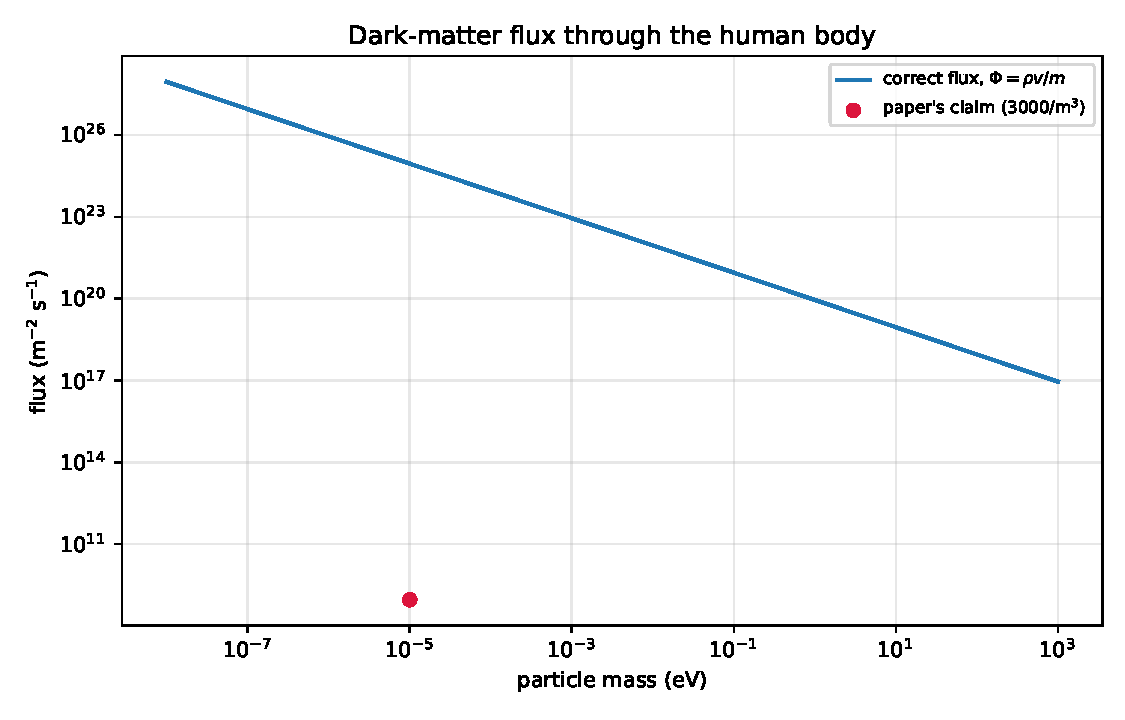
\includegraphics[width=0.82\textwidth]{figures/fig07_flux.pdf}
\caption{The flux of dark matter through the human body as a function of particle mass. The red point marks the claim made in version 30; the curve is the correct value for $\rho = 0.3$ GeV/cm$^3$ and $v = 300$ km/s. At $10^{-5}$ eV the difference is 16 orders of magnitude.}
\label{fig:flux}
\end{figure}

\subsection{What happens to these particles?}
Most of them pass through you without interacting. A few interact with atomic nuclei: spin-independent ($\sim 5$ collisions/year), spin-dependent ($\sim 30$ collisions/year). The effect on the body: natural radiation ($\sim 2.4$ mSv/year); dark matter ($\sim 10^{-15}$ mSv/year).

\subsection{How do we detect these particles?}
Direct detectors: LUX-ZEPLIN (10 tonnes of xenon) --- sensitivity: $10^{-48}$ cm$^2$. Indirect detectors: Fermi-LAT (looking for gamma rays from annihilation), ADMX (looking for axions). Cross-section: $\sigma \sim 10^{-47}$ cm$^2$. Interaction probability: $P \sim 10^{-22}$.

\subsection{Dark matter as a wave, not as particles}
If dark matter is a scalar field, then it is not made of individual particles. It is a wave that fills the universe. Formalisation: $A(x,t) = \sum_n A_n \cos(\omega_n t + \varphi_n)$.

\subsection{The analogy of the tree and the photon}
Imagine a tree on a beach. The Sun is shining. Photons leave the Sun with energy $E = h\nu$. They reach the tree. They are absorbed by every leaf with the same energy $h\nu$. How can a single photon reach all the leaves with the same energy? If it were a particle it would lose energy at every collision. But it does not. The answer is simple: because the photon is a wave, not a particle. A wave is not ``consumed'' as it passes through matter. It spreads across all of space. Every leaf ``sees'' the whole wave. The state of the photon: $|\psi_{\text{photon}}\rangle = \int d^3k \, c(k) |k\rangle$.

\subsection{Wave--particle duality as a traversal mechanism}
If matter cannot cross between universes (because that would require infinite energy) and the universes are connected through dark matter, then how do they communicate? The ART-12D answer: through wave--particle duality. Step 1: matter becomes a wave. $|\text{particle}\rangle_A \to |\text{wave}\rangle_A$. Step 2: the wave crosses over. $|\text{wave}\rangle_A \to |\text{wave}\rangle_B$. Step 3: the wave becomes a particle. $|\text{wave}\rangle_B \to |\text{particle}\rangle_B$. Step 4: the information is transduced. $I_A \to I_B$.

\subsection{The human emotional spectrum}
Human feelings fall into two broad categories: positive and negative. Each feeling has a characteristic frequency and a specific effect on consciousness. Formalisation: $S_{\text{total}} = \sum_{i=1}^{48} S_i^{\text{positive}} + \sum_{j=1}^{46} S_j^{\text{negative}}$. Here is an extract from the extended table (the full version is given in Appendix B):
\begin{table}[H]
\centering
\begin{tabular}{@{}lll@{}}
\toprule
\textbf{Feeling} & \textbf{Dominant frequency (Hz)} & \textbf{Effect} \\ \midrule
Joy & 400-600 & Expansion, dynamism \\
Peace & 200-350 & Reflective calm \\
Love & 200-400 & Deep emotion \\
Gratitude & 300-500 & Contentment \\
Fear & 500-800 & Activates the amygdala \\
Anger & 600-800 & Rage \\
Sadness & 400-600 & Melancholy \\
Envy & 600-800 & Jealousy \\ \bottomrule
\end{tabular}
\end{table}
The therapeutic musical frequencies (432 Hz, 528 Hz, 639 Hz, 741 Hz, 852 Hz, 963 Hz) have been correlated with the frequencies of the akashic field. The seven human senses comprise five physical ones (sight, hearing, smell, taste, touch) and two mental ones (imagination, empathy).

\subsection{The heart as a modulator of reception}
The heart has an electrical system of its own (the sinoatrial node) that generates impulses independently of the brain. It works as a modulator of reception, not as an independent receiver. The brain is the principal receiver, the heart adjusts the coherence. Formalisation: $C_{\text{coherent}} = C_0 \times (1 + \beta \times HRV)$. The exact scientific figures: the brain consumes about $20$ W of metabolic power, the heart delivers about $1-1.3$ W of mechanical power but produces electric and magnetic fields of much larger amplitude.

\subsection{The word that can replace any medicine}
The hypothesis: $L_{\text{word-matter}} = g_{CM} A_{\text{meaning}} \psi \psi$. What the word can do: $Effect_{\text{total}} = Effect_{\text{medicine}} + Effect_{\text{word}} + \text{Interaction}$. What the word cannot do: it cannot replace antibiotics for bacterial infections, it cannot replace insulin for type 1 diabetes, it cannot replace surgery for appendicitis, it cannot replace chemotherapy for cancer. Prediction 67: the effect of the word.

\newpage
